\section{Study Settings}

% Discutir a organizacao geral do nosso
% estudo de caso, em particular qual o objetivo
% que temos. Em termos de um GQM, aqui poderia
% ser incluido o objetivo e as questoes de pesquisa. 

% ver artigos:
% 
% - http://people.irisa.fr/Edward-Mauricio.Alferez_Salinas/REJ/10.1007_s00766-013-0184-5.pdf
% - http://www.les.inf.puc-rio.br/opus/docs/pubs/2013/2013-02.pdf
% - http://www.les.inf.puc-rio.br/opus/docs/pubs/2012/2012-16.pdf
% - http://www.les.inf.puc-rio.br/opus/docs/pubs/2012/2012-03.pdf

\subsection{Case Study: \texttt{IRIS} email client}

%
% discutir um pouco da arquitetura
% quais features foram implementadas inicialmente
% linhas de codigo e outras metricas.
%

%
% discutir um pouco da arquitetura
% quais features foram implementadas inicialmente
% linhas de codigo e outras metricas.
%

The \texttt{IRIS} email client is a Java Standard Edition, version 7 (JSE7), Application. The following features were implemented in the base version:

\begin{itemize}
\item{Send and Receive e-mail messages.}
\item{Multiple folders (though is not possible to create new folders).}
\item{Address Book.}
\item{Relational Database.}
\item{Text-Based User Interface.}
\item{GMail Provider, through IMAP.}
\end{itemize}

\begin{figure}[!ht]
\centering
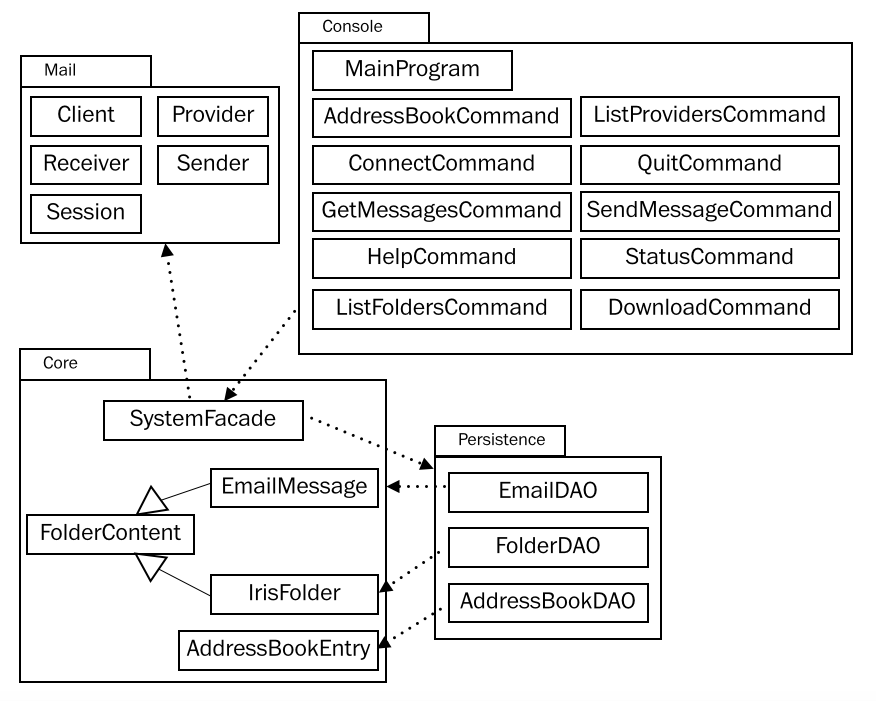
\includegraphics[width=4.5in]{case_study_fig_1.png}
\caption{\texttt{IRIS} Architecture. (UML Notation)}
\label{fig:case_study_fig1}
\end{figure}

The Figure~\ref{fig:case_study_fig1} depicts a simplified view of \texttt{IRIS} architecture. It is decomposed in four packages, namely:

\begin{itemize}
\item{Core: holds the model classes and the fa\c{c}ade.}
\item{Mail: takes care of connecting on providers, send and receiving email messages.}
\item{Persistence: as of base version, implements relational persistence.}
\item{Console: has the entry point of application, and provides commands that allows user to interact with it.}
\end{itemize}

As can be seen on Figure~\ref{fig:case_study_fig1}, the \texttt{SystemFacade} class orchestrates the workflow initiated by the user by issuing a command. Its interactions typically involve calls to \texttt{Mail} and \texttt{Persistence} packages. Note that the \texttt{Console} package are allowed to access only the \texttt{SystemFacade}. The commands classes, by the way, are loaded dinamically by the \texttt{MainProgram}. It searches through the classpath seeking Command interface implementers.

The Multiple Folder feature was implemented in a limited way. Only the \texttt{INBOX} and \texttt{OUTBOX} folders are supported, and are automatically created. By folders, we mean local folders. It must not be confounded with remote folders, that resides on the IMAP server database.

Table~\ref{table:case_study_tab1} shows an overview of the source code metrics of \texttt{IRIS}. All metrics are in good shape, except for Number of Methods by Class and Height of Inheritance Tree, that are outside industry-standard ranges.

\begin{table}[!ht]
%% increase table row spacing, adjust to taste
\renewcommand{\arraystretch}{1.3}
% if using array.sty, it might be a good idea to tweak the value of
% \extrarowheight as needed to properly center the text within the cells
\caption{\texttt{IRIS} metrics}
\label{table:case_study_tab1}
\centering
%% Some packages, such as MDW tools, offer better commands for making tables
%% than the plain LaTeX2e tabular which is used here.
\begin{tabular}{|c|c|c|}
\hline
Metric & Value & Mean Value\\
\hline
LOC & 3035 & 4.87, by method\\
\hline
Methods & 623 & 9.88, by class \\
\hline
Classes & 63 & 3.31, by package \\
\hline
Packages & 19 & \\
\hline
Cyclomatic complexity & 640 & 0.21, by LOC \\
\hline
Fan Out & 453 & 0.59, by call \\
\hline
Calls & 757 & 1.21, by method \\
\hline
Number of Direct Descendants & 0.11 & \\
\hline
Height of inheritance tree & 0.37 & \\
\hline
\end{tabular}
\end{table}

\subsection{First Sprint: extract product line}

\subsection{Second Sprint: Initial evolution of the product line}

% quais features foram introduzidas
% caracterizar o cenario de acordo com o trabalho da Lais Neves em gpce 2011

\subsection{Third Sprint: Final evolution of the product line}


% quais features foram introduzidas
% caracterizar o cenario de acordo com o trabalho da Lais Neves em gpce 2011


\subsection{Metrics and Tools}

% ok, acho que aqui poderiamos discutir nossas metricas de interesse.
% acho que poderiamos focar em acoplamento (ver se Lattix oferece algo),
% estabilidade do codigo, analise de impacto considerando artefatos alterados, artefatos adicionados e
% artefatos removidos. Lembrar que temos interesse em aspectos de configuracao: discussao sobre
% a decomposicao entre Persistencia e AddressBook (acho que com AOP, ficou mais modular, mais facil
% de configurar, etc.)

% descrever tambem as ferramentas e procedimentos usados na medicao. 
